
%(BEGIN_QUESTION)
% Copyright 2008, Tony R. Kuphaldt, released under the Creative Commons Attribution License (v 1.0)
% This means you may do almost anything with this work of mine, so long as you give me proper credit

Shown here is the response of a process to a single step-change on the controller output (made with the controller in ``manual'' mode).  Based on your observations, determine the steady-state gain ($K$), dead time ($L_R$), and reaction rate ($R_R$):

$$\includegraphics[width=15.5cm]{i01657x01.eps}$$

$K$ = \underbar{\hskip 50pt} \hskip 50pt $L_R$ = \underbar{\hskip 50pt} \hskip 50pt $R_R$ = \underbar{\hskip 50pt}

\vskip 10pt

Also, determine whether the controller will need to be configured for {\it direct} or {\it reverse} action to successfully control this process.

\underbar{file i01657}
%(END_QUESTION)





%(BEGIN_ANSWER)

$$\includegraphics[width=15.5cm]{i01657x02.eps}$$

\medskip 
\item{}Steady-state gain ($K$) = 2
\vskip 5pt
\item{}Dead time ($L_R$) = 0.25 minutes
\vskip 5pt
\item{}Reaction rate ($R_R$) = 3.2\% / unit-minute
\end{itemize} 

\vskip 10pt

Note: the unit of ``unit-minute'' for reaction rate refers to reaction rate corrected for percentage of output step.  In other words, this is not the raw reaction rate figure, but rather the reaction rate per percent of output step.

\vskip 10pt

This controller must be configured for {\bf direct} action in order to control this process.

%(END_ANSWER)





%(BEGIN_NOTES)

The fact that the process is ``reverse'' acting instead of ``direct'' is of no consequence in calculating process gain, dead time, reaction rate, or time constant.

%INDEX% Control, PID tuning: step change (output) revealing process gain
%INDEX% Control, PID tuning: step change (output) revealing process dead time
%INDEX% Control, PID tuning: step change (output) revealing process reaction rate

%(END_NOTES)


